\documentclass[urlcolor=blue,dvipsnames]{beamer}

\usepackage[utf8]{inputenc}
\usepackage{fancybox,fancyvrb}
\usepackage{environ,xspace,empheq}

\usepackage{tikz}
\usetikzlibrary{arrows.meta,decorations.markings,decorations.pathreplacing,fadings,positioning}

\hypersetup{colorlinks,linkcolor=,urlcolor=cyan}

\beamertemplatenavigationsymbolsempty
\setbeamertemplate{footline}[frame number]
\usetheme{Pittsburgh}

\newcommand\enumnum[1]{{\renewcommand{\insertenumlabel}{#1}%
      \usebeamertemplate{enumerate item} \,}}

\newcommand{\grad}{\nabla}
\newcommand{\ih}{\boldsymbol{\hat{\textbf{\i}}}}
\newcommand{\jh}{\boldsymbol{\hat{\textbf{\j}}}}
\newcommand{\vF}{\boldsymbol{\vec{\textbf{F}}}}
\newcommand{\Matlab}{\textsc{Matlab}\xspace}
\newcommand{\Octave}{\textsc{Octave}\xspace}


\title{7.2 \emph{inverse} Laplace Transforms \\ (and use of $\mathcal{L}$ for DEs)}

\subtitle{a lesson for MATH F302 Differential Equations}

\author{Ed Bueler, Dept.~of Mathematics and Statistics, UAF}

\date{\tiny \today}


\begin{document}
\setbeamertemplate{itemize item}{$\bullet$}
\setbeamertemplate{itemize subitem}{$\circ$}
\renewcommand{\thefootnote}{{\color{green} \arabic{footnote}}}

\begin{frame}
\titlepage

\centerline{\tiny for textbook: \, D. Zill, \emph{A First Course in Differential Equations with Modeling Applications}, 11th ed.}
%\color{green!40!blue}
\end{frame}

\newcommand{\LL}[1]{\mathcal{L}\left\{#1\right\}}

\begin{frame}{recall the definition}

\begin{itemize}
\item the \emph{Laplace transform} of a function $f(t)$ defined on $(0,\infty)$ is
    $$\LL{f(t)} = \int_0^\infty e^{-st} f(t)\,dt$$
    \begin{itemize}
    \item this is well defined for $s>c$ if $f(t)$ has exponential order $c$:  $|f(t)| \le M e^{ct}$
    \end{itemize}

\bigskip
\item the result of applying the Laplace transform is a function of s:
    $$\LL{f(t)} = \LL{f}(s) = F(s) \hspace{15mm} \longleftarrow \text{all mean the same}$$
\end{itemize}
\end{frame}


\begin{frame}{the Laplace transform strategy}

\begin{center}
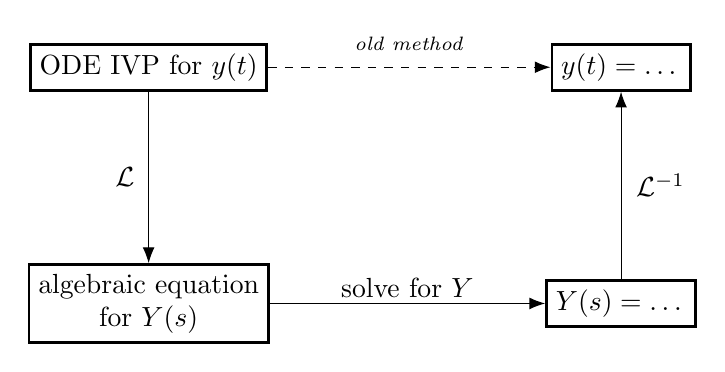
\begin{tikzpicture}[scale=1.0,>={Latex[length=2mm]},
  component/.style={rectangle,draw,fill=white,align=center,line width=1pt}]

\draw (-3,3) node[component] (ode) {ODE IVP for $y(t)$};
\draw (-3,0) node[component] (Leqn) {algebraic equation \\ for $Y(s)$};
\draw (3,0) node[component] (Lsoln)   {$Y(s)=\dots$};
\draw (3,3) node[component] (odesoln)   {$y(t)=\dots$};
\path
   (ode) edge[->] node[xshift=-3mm] {$\mathcal{L}$} (Leqn)
   (Leqn) edge[->] node[yshift=2mm] {solve for $Y$} (Lsoln)
   (Lsoln) edge[->] node[xshift=+5mm] {$\mathcal{L}^{-1}$} (odesoln)
   (ode) edge[dashed,->] node[yshift=3mm] {\scriptsize \emph{old method}} (odesoln);

\end{tikzpicture}
\end{center}
\end{frame}


\begin{frame}{Z}

\begin{itemize}
\item X
\end{itemize}
\end{frame}


\begin{frame}{expectations}

\begin{itemize}
\item just watching this video is \emph{not} enough!
     \begin{itemize}
     \item see ``found online'' videos and stuff at

     \centerline{\href{https://bueler.github.io/math302/week11.html}{\tt \color{cyan} bueler.github.io/math302/week11.html}}
     \item \emph{read} section 7.2 (and 7.1 and 7.3) in the textbook
     \item \emph{do} the WebAssign exercises for section 7.2
     \end{itemize}
\end{itemize}
\end{frame}

\end{document}

